\section{Safety of Autonomous Vehicle}
\label{sec:av_safety}

Autonomous vehicle is a good example of a safety critical and time critical system. All the modules in an AV must work in absolute sunchronocity to ensure the safety of the vehicle. It is often necessary to provide formal guarantees on the safety of the AV. However, it is often difficult to verify complex systems like an AV that is composed of several interacting components. This problem is further exacerbated by the fact that AVs often use ANNs as controllers (the LCD module in this case study). ANNs are known to be difficult to verify due to their non-linear nature and their large (often infinite) input-output space.

One solution to this problem is to use compositional Assume-Guarantee reasoning. Assume-Guarantee reasoning is a formal method that assumes conditions and gurantees conditions. Moreover, compositional reasoning is a technique that allows us to reason about the system as a composition of its components. This allows us to reason about the system in a modular way, and to verify the system by verifying its components. This is particularly useful in the case of AVs, where the system is composed of several interacting components.

\begin{figure}[htbp]
    \centering
    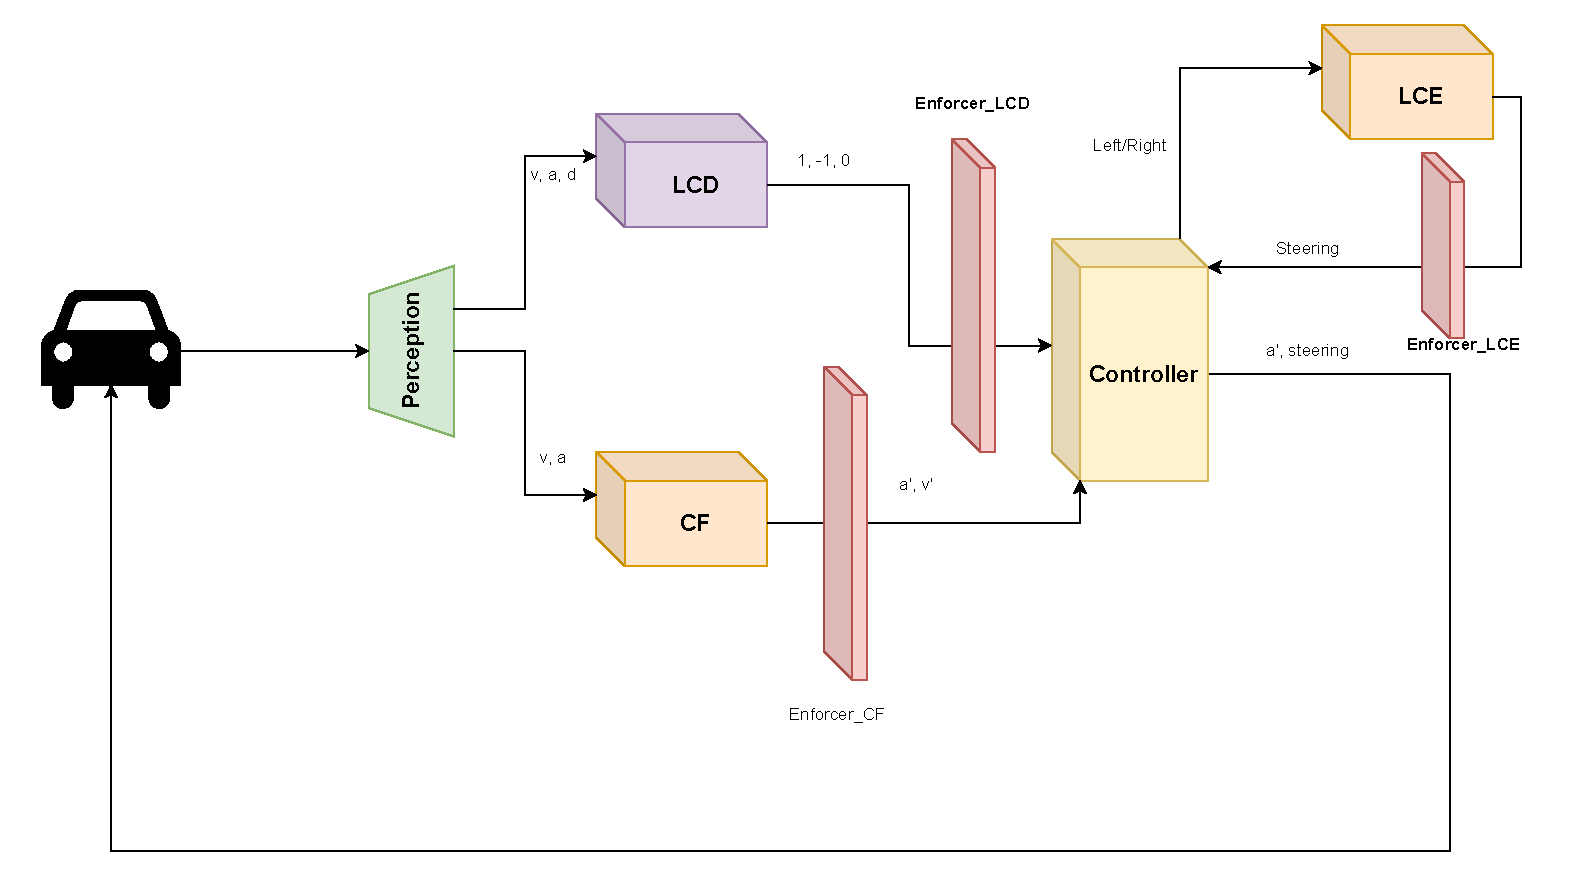
\includegraphics[width = \linewidth]{sections/av/fig/AV_full_enforcer.pdf}
    \caption{AV case study with runtime enforcement}
    \label{fig:av_runtime_enforcement}
\end{figure}

In this case study, we assume the satisfaction of certain properties to guarantee the safety of the AV. To ensure that the properties are satisfied, we do not use formal verification approaches and rather use runtime enforcement techniques. Runtime enforcement is a technique that ensures that the system satisfies certain properties at runtime. It does this by monitoring the system at runtime, and by enforcing certain constraints on the system. If the system violates the constraints, the runtime enforcement mechanism takes corrective actions to bring the system back to a safe state. 

We add enforcers at the outputs of all three modules to ensure that the controller gets correct output to be passed onto the car controls. We do not need another enforcer for the controller as the inputs to the controller are being corrected to satisfy safety properties. As long as the controller and the properties are specified correctly, the car should recieve safe inputs to work on. 

Furthermore, we would like to ensure that the enforcer correction should not happen too often. To achieve this, we also propose a compositional policy-driven training of the models based on a novel policy mining technique. The training ensures that the models adhere to mined polcies with certain accuracy. The following sections describe enforcement, the safety policies and the compositional training in detail.



